\documentclass[12pt]{article}
\usepackage{amsmath}
\usepackage{graphicx,psfrag,epsf}
\usepackage{enumerate}
\usepackage{natbib}
\usepackage{float}
\usepackage{blindtext}
\usepackage{hyperref}
\usepackage{booktabs,dcolumn}
\usepackage{indentfirst}
\usepackage{caption}
\usepackage{hyperref}
\usepackage{appendixnumberbeamer}
\usepackage{multicol}
\usepackage{booktabs}
\usepackage{outlines} % new package, delete if getting package errors
\usepackage[scale=2]{ccicons}
\usepackage{graphicx}
\usepackage{pgfplots}
\usepgfplotslibrary{dateplot}
\usepackage{subcaption}
\captionsetup{compatibility=false}
\usepackage{xspace}
\usepackage{tikz}
\usepackage{newtxtext}
\usepackage{titlesec}
\usepackage{lscape}
\hypersetup{
    colorlinks=true,
    linkcolor=blue,
    filecolor=magenta,      
    urlcolor=cyan,
}
\newcolumntype{d}{D{.}{.}{2.5}}           % alignment on decimal marker
\newcommand\mc[1]{\multicolumn{1}{c}{#1}}
\usepackage{url} % not crucial - just used below for the URL 

%\pdfminorversion=4
% NOTE: To produce blinded version, replace "0" with "1" below.
\newcommand{\blind}{0}

% DON'T change margins - should be 1 inch all around.
\addtolength{\oddsidemargin}{-1in}%
\addtolength{\evensidemargin}{-1in}%
\addtolength{\textwidth}{1in}%
\addtolength{\textheight}{1.3in}%
\addtolength{\topmargin}{-.8in}%

\doublespacing
\begin{document}

%\bibliographystyle{natbib}

\def\spacingset#1{\renewcommand{\baselinestretch}%
{#1}\small\normalsize} \spacingset{1}


%%%%%%%%%%%%%%%%%%%%%%%%%%%%%%%%%%%%%%%%%%%%%%%%%%%%%%%%%%%%%%%%%%%%%%%%%%%%%%

\if0\blind
{
  \title{\bf Turkish Elections and Catastrophic Events}
    {
}

  \maketitle
} \fi

\if1\blind
{
  \bigskip
  \bigskip
  \bigskip
  \begin{center}
    {\LARGE\bf Title}
\end{center}
  \medskip
} \fi

\spacingset{1.45} % DON'T change the spacing!
\section{Introduction}
\label{sec:intro}

A year ago, Turkey celebrated a century of being a democracy. Now, only 2 years away from the same milestone for being a republic, it is inevitable to think and analyse the trends of Turkish democracy. 
It is reasonable to say, Turkey, which resides possibly one of the lesser stable regions in the world; suffered a lot during this period, while trying to establish their democratic traditions. Having survived 3 coups, 3 "soft" coups and numerous economic, political and civil crises, Turkey still maintained regular and somewhat fair elections without interruption, unlike many other countries in a similar political landscape. The goal of this paper is to materialise this continuity and uncover the impact of catastrophic events in Turkey to voting behavior and results. 

\section{Background}

\subsection{Brief Summary of Turkish History}

After the end of World War I, like many empires in Europe; Ottoman Empire crumbled. In it's heartland, Turkey emerged as a new republic in 1923 after a long period of successive independence war against the colonial powers. 

Founded as a parliamentary republic, the first 17 years of the country has been defined by a single party period in which the founding party Republican People's Party, (Turkish abbreviation CHP will be used thereafter) was in power. The party is defined by having pro-European, Liberal and Secular values. Only in 1950, Turkey had it's truly first election with emergence of Right wing parties. Between 1950 - 2018, Turkey remained as a parliamentary republic with periodic municipal and parliamentary elections.

In 2018, with a 51\% referendum result, Turkey decided to transition into a presidential republic where the president and the Parliament is elected at the same time, using different ballots. For this project's scope Turkey's only 2 presidential elections were excluded from research. 

Inheriting many problems of it's predecessor, since it's foundation Turkey needed to deal with both regional and domestic problems. Composed of many different ethnic backgrounds such as Turkish, Kurdish, Armenian, Zaza etc. Turkey had to actively fight to maintain it's regional integrity. Moreover, as the gateway of Middle East to Europe, Turkey suffered from many regional events taking place outside of it's borders. One great example of this is the refugee influx to Turkey after ISIS war in Syria in 2011. 

\subsection{Summary of Catastrophic Events}

The research consists of 4 main catastrophic events, which will be used to analyze voter behaviour. 

\subsubsection{1999 Marmara Earthquake}
On August 17, 1999 the Marmara Region in Turkey was devastated from a 7.5 magnitude earthquake that lasted for several days. Most of the buildings in the epicenter of the earthquake were either severely damaged or collapsed by the end of the event. Approximately 18,000 people were killed. It was a showcase of Turkey's unpreparedness for earthquakes, a country which sits on various earthquake lines.

\begin{subfigure}[t]{.49\textwidth}
    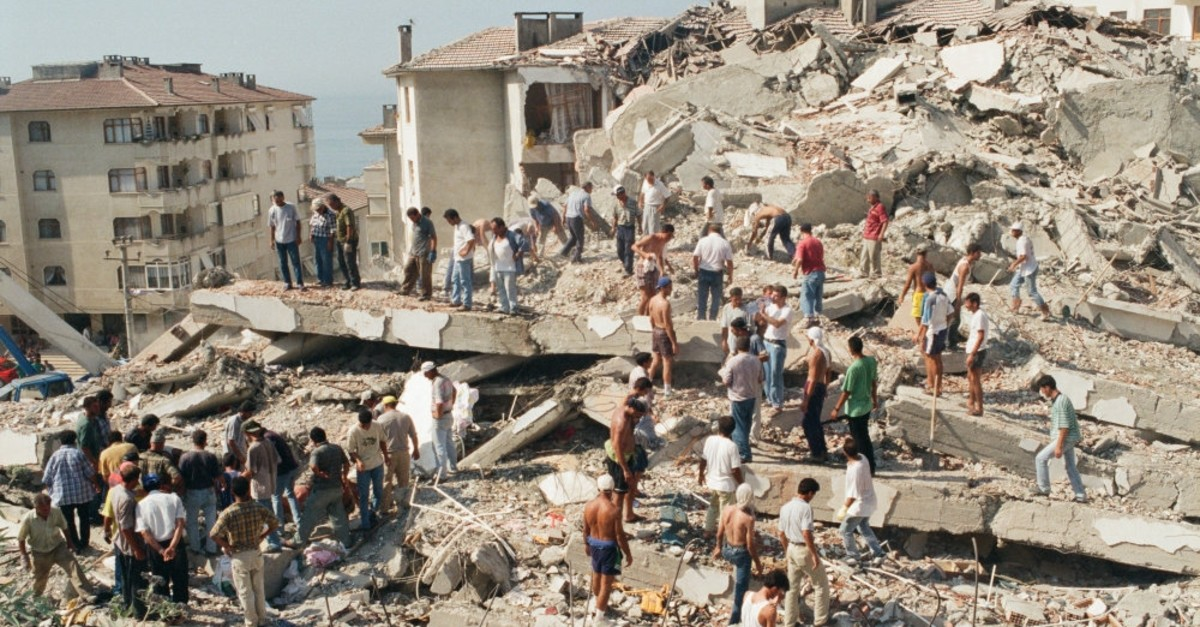
\includegraphics[scale=0.15]{paper/figures/earthquake_marmara2.jpeg}
	\caption{Marmara Earthquake}
	\end{subfigure}
	\begin{subfigure}[t]{.49\textwidth}
    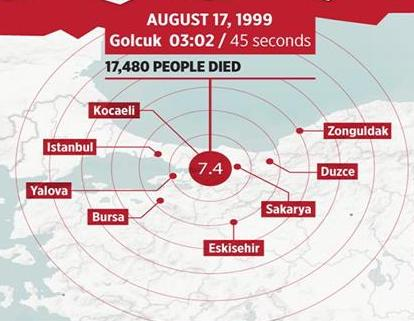
\includegraphics[scale=0.3]{paper/figures/marmara_affected.jpeg}
	\caption{Regions Affected}
\end{subfigure}

\subsubsection{1974 Cyprus Peace Operation}

The island of Cyprus, which used to be ruled entirely by Republic of Cyprus lies in the Eastern Mediterranean, approximately 70km away from the Turkish mainland. The island is composed of Cypriot Greeks and Cypriot Turks. While the latter is the minority, the founding principles of the Republic of Cyprus ensured equal representation for both, and assigned Turkey, Greece and the UK as guarantor states. All had the ability to intervene if the ethnic groups they represent were in danger. The tension in the island was ever increasing with Turkish minority under attack by Greek Nationalist organizations but the tipping point was in 1974; when a pro Greek unification president got elected in the island. 

Turkey decided to intervene, causing relocation of many Greek and Turkish locals and separation of the island into 2. The north declared it's independence as Turkish Republic of Northern Cyprus; which is only recognized by Turkey. 

\subsubsection{2011 Refugee Crisis}

In 2011, a civil war started in Syria after a set of peaceful student demonstrations caused the government's crackdown. 80\% of the Syrians got displaced and the majority of them entered to Turkey via the border, making Turkey the largest refugee holder in the world since 2014. 

\subsubsection{1984 Conflict with Kurdish Armed Groups}

Composing one fifth of Turkey's population, ethnic Kurdish people mostly live in the Eastern cities in Turkey (mainly Van, Diyarbakir). The PKK (Kurdish Worker's Party), established by Abdullah Ocalan in 1978, has waged an insurgency since 1984 against Turkish authorities for greater cultural and political rights, primarily with the objective of establishing an independent Kurdish state. The ongoing conflict in the eastern region has resulted in nearly forty thousand deaths. The organization has been labelled as a terrorist organization by Turkey and it's allies. 


\section{Data and Summary Statistics}

The data is retrieved retrieved from Turkish Statistical Institute, which is the main source for census and election data in Turkey. It consists 139 municipal and 264 parliamentary election results on a city and year level. The main columns of interest are the election year, city, election type, percentage turnout, winning party and the vote share, previous winning party and vote share. 



The process of data cleaning and creation can be found in the author's \href{https://github.com/deniztokmakoglu/turkish_election_analysis}{github page.}



\section{Research Design}

The main research goal of this paper is to uncover effects of regional crises on voter behavior. To define voter behaviour, percentage turnout and the vote share of the winning party is used. 

The research follows Difference in Difference design where each city got affected by an event is compared wit itself (pre-event and post-event) and other cities in the country that has not been effected by an event. The regression format is as follows;

$$ Y_i = \beta_{1} + {event * post\_event} + \beta_{2} * {event} + \beta_{3} * {post\_event} + \theta_i$$

Where $Y_i$ is the outcome of interest and $\theta_i$ is year, city and election type fixed effects.

To make the catastrophic event more relevant with election results, only the preceding 2 and suceeding 2 elections were considered in the analysis.

The research is conducted in three levels:

\subsection{Voter Turnout}

On this level, the outcome of interest is Voter Turnout and the regression is conducted for the entire sample. This is to understand whether catastrophic events change voter confidence in democracy or make elections a matter of 'life and death'.

\subsection{Outcome}

For this level, 2 outcome of interests are present. First, whether to see if the city punishes the ruling party after a catastrophic event. This can be tracked by comparing the winner of the election with the previous winner to see if there is a swing.

The second outcome of interest is the level of incumbent vote for cities that did not change the ruling party after an event. This is to understand how much the voter values the government's response to a catastrophic event which is explained by the difference in the vote share of the continuing ruling party.

\subsection{Heterogeneous Event Effects}

The third level of the analysis is to uncover the specific effects of each (type) of event on vote outcome and voter turnout. This is potentially to understand what type of events speak to the Turkish voters and uncover regional differences in response to the same type of events.

\section{Results and Discussion}

\subsection{Voter Turnout}

As results indicate on Table A1, an event does not change voter tendency to vote. This can indicate that Turkish belief in democratic institutions does not change with a catastrophic event. This is to be expected as traditionally, Turkish turnout in voting is always one of the highest in the world.

\subsection{Vote Outcome}

From table A2, it appears that the vote share of the same ruling party increases by 6\% after a catastrophic event. This means cities that experienced a catastrophic event puts event more faith into the ruling party. This can also potentially be explained by the 'rallying' effect of wars. Yet, this result is also expected as Turkish voters historically lost faith in the ruling party only after economic crises, which is not included in the scope of this research. 

Arguably, Table A3 suggests that cities do not swing after a catastrophic event, which means the voter is not punishing the incumbent party for the event. 


\subsection{Heterogeneous Event Effects}

The 'rallying' effect' is clearly visible under table A4 as the vote share of the incumbent is increased by 17 and 15 percent respectively after Kurdish Armed Conflict and Cyprus Peace Operation events. 
One thing to note though, the regions effected by Kurdish Armed Conflict are traditionally ruled by parties that also have Kurdish identities. Therefore, the change in vote share might be explained as political efforts to legitimize Kurdish presence. This however, does not imply that the military operations and parties with Kurdish tendencies have anything to do with one another.  

Conversely, according to table A5, voter turnout in cities affected by the Kurdish Armed Conflict was 4 percent less than other cities. One possible explanation is that after armed conflict; some supporters of increased autonomy for Kurdish people might have lost faith in the democratic means of representation. Another possible explanation is the same people might have lost confidence in the cause as they would have thought armed conflict is not the way to gain further rights.

Finally, Syrian Refugee crisis increased the voter turnout by 3 percent in the affected cities. 
\newpage
\section{Appendix}
\captionsetup[table]{name=Table A}
\begin{table}[!htbp] \centering 
  \caption{Effects of a Catastrophic Event on Voter Turnout} 
  \label{} 
\begin{tabular}{@{\extracolsep{5pt}}lc} 
\\[-1.8ex]\hline 
\hline \\[-1.8ex] 
 & \multicolumn{1}{c}{\textit{Dependent variable:}} \\ 
\cline{2-2} 
\\[-1.8ex] &  \\ 
 & Voter Turnout \\ 
\hline \\[-1.8ex] 
 Treatment Effect & 0.640 \\ 
  & (0.650) \\ 
  & \\ 
\hline \\[-1.8ex] 
Observations & 200 \\ 
R$^{2}$ & 0.894 \\ 
Adjusted R$^{2}$ & 0.855 \\ 
Residual Std. Error & 2.697 (df = 146) \\ 
\hline 
\hline \\[-1.8ex] 
\textit{Note:}  & \multicolumn{1}{r}{$^{*}$p$<$0.1; $^{**}$p$<$0.05; $^{***}$p$<$0.01} \\ 
\end{tabular} 
\end{table} 


\begin{table}[!htbp] \centering 
  \caption{Effects of a Catastrophic Event on Incumbent Vote Share} 
  \label{} 
\begin{tabular}{@{\extracolsep{5pt}}lc} 
\\[-1.8ex]\hline 
\hline \\[-1.8ex] 
 & \multicolumn{1}{c}{\textit{Dependent variable:}} \\ 
\cline{2-2} 
\\[-1.8ex] &  \\ 
 & Incumbent Vote Share \\ 
\hline \\[-1.8ex] 
 Treatment Effect & 6.310$^{***}$ \\ 
  & (2.133) \\ 
  & \\ 
\hline \\[-1.8ex] 
Observations & 117 \\ 
R$^{2}$ & 0.863 \\ 
Adjusted R$^{2}$ & 0.759 \\ 
Residual Std. Error & 5.848 (df = 66) \\ 
\hline 
\hline \\[-1.8ex] 
\textit{Note:}  & \multicolumn{1}{r}{$^{*}$p$<$0.1; $^{**}$p$<$0.05; $^{***}$p$<$0.01} \\ 
 & \multicolumn{1}{r}{Only elections with non-swing result are considered.} \\ 
\end{tabular} 
\end{table} 

\begin{table}[!htbp] \centering 
  \caption{Effects of a Catastrophic Event on Change in Leadership} 
  \label{} 
\begin{tabular}{@{\extracolsep{5pt}}lc} 
\\[-1.8ex]\hline 
\hline \\[-1.8ex] 
 & \multicolumn{1}{c}{\textit{Dependent variable:}} \\ 
\cline{2-2} 
\\[-1.8ex] &  \\ 
 & Dummy for Leadership Change \\ 
\hline \\[-1.8ex] 
 Treatment Effect & $-$0.040 \\ 
  & (0.080) \\ 
  & \\ 
\hline \\[-1.8ex] 
Observations & 200 \\ 
R$^{2}$ & 0.668 \\ 
Adjusted R$^{2}$ & 0.548 \\ 
Residual Std. Error & 0.332 (df = 146) \\ 
\hline 
\hline \\[-1.8ex] 
\textit{Note:}  & \multicolumn{1}{r}{$^{*}$p$<$0.1; $^{**}$p$<$0.05; $^{***}$p$<$0.01} \\ 
\end{tabular} 
\end{table} 
\begin{table}[!htbp] \centering 
  \caption{Effects of a Catastrophic Event on Incumbent Vote Share} 
  \label{} 
\begin{tabular}{@{\extracolsep{5pt}}lcccc} 
\\[-1.8ex]\hline 
\hline \\[-1.8ex] 
 & \multicolumn{4}{c}{\textit{Dependent variable:}} \\ 
\cline{2-5} 
\\[-1.8ex] & \multicolumn{4}{c}{Incumbent Vote Share} \\ 
\\[-1.8ex] & (1) & (2) & (3) & (4)\\ 
\hline \\[-1.8ex] 
 Kurdish Armed Conflict & 28.609$^{***}$ &  &  &  \\ 
  & (7.097) &  &  &  \\ 
  & & & & \\ 
 Marmara Earthquake &  & 5.044 &  &  \\ 
  &  & (4.238) &  &  \\ 
  & & & & \\ 
 Cyprus Peace Operation &  &  & 20.260$^{***}$ &  \\ 
  &  &  & (5.659) &  \\ 
  & & & & \\ 
 Syrian Refugees &  &  &  & $-$1.129 \\ 
  &  &  &  & (5.580) \\ 
  & & & & \\ 
\hline \\[-1.8ex] 
Observations & 117 & 117 & 117 & 117 \\ 
R$^{2}$ & 0.875 & 0.848 & 0.870 & 0.845 \\ 
Adjusted R$^{2}$ & 0.781 & 0.733 & 0.771 & 0.727 \\ 
Residual Std. Error (df = 66) & 5.575 & 6.158 & 5.695 & 6.221 \\ 
\hline 
\hline \\[-1.8ex] 
\textit{Note:}  & \multicolumn{4}{r}{$^{*}$p$<$0.1; $^{**}$p$<$0.05; $^{***}$p$<$0.01} \\ 
 & \multicolumn{4}{r}{Only elections with non-swing result are considered.} \\ 
\end{tabular} 
\end{table} 

\begin{table}[!htbp] \centering 
  \caption{Effects of a Catastrophic Event on Voter Turnout} 
  \label{} 
\begin{tabular}{@{\extracolsep{5pt}}lcccc} 
\\[-1.8ex]\hline 
\hline \\[-1.8ex] 
 & \multicolumn{4}{c}{\textit{Dependent variable:}} \\ 
\cline{2-5} 
\\[-1.8ex] & \multicolumn{4}{c}{Voter Turnout} \\ 
\\[-1.8ex] & (1) & (2) & (3) & (4)\\ 
\hline \\[-1.8ex] 
 Kurdish Armed Conflict & $-$4.329$^{**}$ &  &  &  \\ 
  & (1.905) &  &  &  \\ 
  & & & & \\ 
 Marmara Earthquake &  & 1.247 &  &  \\ 
  &  & (1.144) &  &  \\ 
  & & & & \\ 
 Cyprus Peace Operation &  &  & 1.450 &  \\ 
  &  &  & (1.723) &  \\ 
  & & & & \\ 
 Syrian Refugees &  &  &  & 2.266 \\ 
  &  &  &  & (1.772) \\ 
  & & & & \\ 
\hline \\[-1.8ex] 
Observations & 200 & 200 & 200 & 200 \\ 
R$^{2}$ & 0.893 & 0.890 & 0.890 & 0.890 \\ 
Adjusted R$^{2}$ & 0.855 & 0.851 & 0.850 & 0.851 \\ 
Residual Std. Error (df = 147) & 2.698 & 2.734 & 2.739 & 2.730 \\ 
\hline 
\hline \\[-1.8ex] 
\textit{Note:}  & \multicolumn{4}{r}{$^{*}$p$<$0.1; $^{**}$p$<$0.05; $^{***}$p$<$0.01} \\ 
\end{tabular} 
\end{table} 

\begin{table}[!htbp] \centering 
  \caption{Effects of a Catastrophic Event on Voter Turnout} 
  \label{} 
\begin{tabular}{@{\extracolsep{5pt}}lcccc} 
\\[-1.8ex]\hline 
\hline \\[-1.8ex] 
 & \multicolumn{4}{c}{\textit{Dependent variable:}} \\ 
\cline{2-5} 
\\[-1.8ex] & \multicolumn{4}{c}{Voter Turnout} \\ 
\\[-1.8ex] & (1) & (2) & (3) & (4)\\ 
\hline \\[-1.8ex] 
 Kurdish Armed Conflict & $-$4.180$^{**}$ &  &  &  \\ 
  & (1.881) &  &  &  \\ 
  & & & & \\ 
 Marmara Earthquake &  & 1.398 &  &  \\ 
  &  & (1.128) &  &  \\ 
  & & & & \\ 
 Cyprus Peace Operation &  &  & 1.588 &  \\ 
  &  &  & (1.699) &  \\ 
  & & & & \\ 
 Syrian Refugees &  &  &  & 3.282$^{*}$ \\ 
  &  &  &  & (1.778) \\ 
  & & & & \\ 
\hline \\[-1.8ex] 
Observations & 200 & 200 & 200 & 200 \\ 
R$^{2}$ & 0.896 & 0.894 & 0.893 & 0.895 \\ 
Adjusted R$^{2}$ & 0.859 & 0.855 & 0.855 & 0.857 \\ 
Residual Std. Error (df = 146) & 2.662 & 2.692 & 2.698 & 2.675 \\ 
\hline 
\hline \\[-1.8ex] 
\textit{Note:}  & \multicolumn{4}{r}{$^{*}$p$<$0.1; $^{**}$p$<$0.05; $^{***}$p$<$0.01} \\ 
\end{tabular} 
\end{table} 

\end{document}

